\documentclass[a4paper,12pt]{article}
\usepackage[utf8]{inputenc}
\usepackage{graphicx}
\usepackage{multicolumn}
\usepackage{multirow}
\usepackage{booktabs}
\usepackage[indent=0pt,skip=3mm]{parskip}
\usepackage{array}
\usepackage{commath} % for abs ||
\usepackage{listings}             % Include the listings-package
\usepackage{tabs}
% \usepackage{colortbl}
% \usepackage{url}
\usepackage{hyperref}
\usepackage{datetime}
\usepackage[ top=5cm, left=1.5cm, right=1.5cm, headheight=4cm,bottom=1cm]{geometry}
\usepackage{lastpage} % include last page numbering
\usepackage{fancyhdr}
\usepackage[table]{xcolor}% ctan.org/pkg/xcolor %FOR COLORS
% \usepackage{frame}
\settimeformat{xxivtime}
\setdefaultdate{\ddmmyyyydate}
\hyphenation{matriz}
\graphicspath{{figures/}{./images/}}
\newcommand{\eq}[1]{$#1$}
\newcommand{\head}[1]{{\bfseries #1}}
\newcommand{\header}[2][\tiny]{{\bfseries #1 #2}}

%%%%%%%%%%%%%%%%%%%%%%%%%%%%%%%%%%%%%%%%%%%%%%%%%%%%%%%%%%%%%%%%%%%%%%
%%%%%%%%%%%%%%%%%%%%%%%%%%%%%%%%%%%%%%%%%
\newsavebox{\mytabularheader}
\newsavebox{\mytabularheadertitle}
\setlength{\extrarowheight}{0.1cm}
%----------------------------------------------------------------------------------
%-----------------------------------------------------------------------------------------------
\sbox{\mytabularheadertitle}{%
  \begin{minipage}{.52\textwidth}
    \begin{center}
        \bfseries \scriptsize  UNIVERSIDAD NACIONAL DE SAN AGUSTIN\\
        FACULTAD DE INGENIERÍA DE PRODUCCIÓN Y SERVICIOS\\
        ESCUELA PROFESIONAL DE INGENIERÍA DE SISTEMA\\[3mm]
    \end{center}
  \end{minipage}
}

\sbox{\mytabularheader}{%
    \begin{minipage}{\textwidth}
        \centering
        \begin{tabular}{cp{8cm}c}
            
\includegraphics[scale=0.3]{epis_logo.png} & 
            \usebox{\mytabularheadertitle} &
            
\includegraphics[scale=0.05]{abet_logo.png} \\
            % \hline
            \multicolumn{3}{c}{Formato: Guía de Práctica de Laboratorio / Talleres / Centros de Simulación}\\
             &\multicolumn{1}{c}{Aprobación:  2022/03/01 Código: GUIA-PRLE-001} &  \\
        \end{tabular}
    \end{minipage}
}
%---------------------------------------
\renewcommand{\headrulewidth}{0pt}
\fancypagestyle{plain}{%
  \fancyhf{}%
  \fancyhf[ch]{\usebox{\mytabularheader}}
}
%--------------------------------------
\pagestyle{plain}
%%%%%%%%%%%%%%%%%%%%%%%%%%%%%%%%%%%%%%%%%%%%%%%%%%%%%%%%%%%%%%%%%%%%%%%%%%%%%%%%%%%%%%%%%%
\definecolor{blackRed}{cmyk}{0,81,76,31}

\begin{document}    
\lstset{language=Python,frame=single, firstnumber=1,basicstyle=\footnotesize,
numbers=left,showspaces=false,showstringspaces=false}   
    \begin{table}[t]
        \centering
        \begin{tabular}{|p{2.3cm}<{:}|m{1.7cm}|m{2.4cm}|m{2cm}|m{3cm}|m{0.6cm}|}
            \multicolumn{6}{c}{\cellcolor{red}{\leavevmode\color{white}\header{INFORMACIÓN BÁSICA}}}\\
            \hline
            \header{ASIGNATURA} & \multicolumn{5}{c}{\header[\footnotesize]{Física Computacional.}}\\
            \hline
            \header{\mbox{TÍTULO DE LA} PRÁCTICA} & \multicolumn{5}{c}{\header[\footnotesize]{Práctica de Ecuación diferencial de Laplace.}}\\
            \hline
            \header{\mbox{NÚMERO DE} PRÁCTICA} & {\header[\footnotesize]{07}} & \header{AÑO LECTIVO:} & {\header[\footnotesize]{2022-A}} & \header{NRO. SEMESTRE:} & \header[\footnotesize]{VII}\\
            \hline
            \header{\mbox{FECHA DE} \mbox{PRESENTACIÓN}} & \header{\today} & \header{HORA DE \mbox{PRESENTACIÓN:}} & \multicolumn{3}{c}{\header[\footnotesize]{\currenttime}}\\
            \hline
            \multicolumn{4}{l}{\header[\footnotesize]{Integrante(s): Alván Ventura Edsel Yael}} & \header{NOTA} & \\
            \hline
            \multicolumn{6}{l}{\header[\footnotesize]{DOCENTE(s):} \header[\footnotesize]{Danny Giancarlo Apaza Veliz.}} \\  
            \bottomrule
        \end{tabular}
    \end{table}
    \title{Práctica 7\\Ecuación de onda\\Física Computacional}
    \date{\vspace{-5ex}}
    \maketitle
    \begin{center}
        Escrito por\\
        Alván Ventura, Edsel Yael\\ \texttt{ealvan@unsa.edu.pe}
        \\[3mm]
        Profesor\\Apaza Veliz, Danny Giancarlo\\ \texttt{dapazav@unsa.edu.pe}\\[3mm]
        \today
    \end{center}
    % \newgeometry{top=2cm}
    \enlargethispage{\baselineskip}
    % \newpage
    \section{Análisis}
    
    A continuación se muestra el análisis de como se llego a la aproximación numérica
    con respecto a la ecuación de onda:
    \begin{equation}
        \frac{\partial^2 u(x,t)}{\partial t^2} = v^2\frac{\partial^2 u(x,t)}{\partial x^2}
    \end{equation}
    \clearpage
    En la siguiente imagen se muestra el análisis de la ecuación de onda:
    \begin{figure}[h]
        \centering
        \includegraphics[width=0.9\textwidth,angle=90]{analisis_1.jpg}
        \caption{Análisis parte 1}
        \label{fig:ana1}
    \end{figure}
    \enlargethispage{\baselineskip}
    \clearpage
    \begin{figure}[t]
        \centering
        \includegraphics[width=\textwidth,angle=180]{analisis_2.jpg}
        \label{fig:ana2}
        \caption{Análisis parte 2}
    \end{figure}

    Como se puede ver en las imágenes anteriores,
    la malla esta constituida al principio de dos valores predeterminados
    que estan evaluados en las funciones \eq{u_0(x)} y \eq{u_1(x)}(figura \ref{fig:ana1}).

    \section{Implementación}
    Para hacer la siguiente implementación se uso:
    \begin{enumerate}
        \item La formula de ecuación de onda en una dimensión.
        \item El lenguaje de programación de Python version 3.
        \item Las libreria \emph{numpy} y la libreria \emph{malplotlib}
    \end{enumerate}

    A continuación se muestra una implementación vertical 
    de la matriz que grafica la ecuación de onda.
    
    \lstinputlisting[title=Archivo de ecuación de Onda]{waveEquation.py}

    \section{Problemas}
    Realice la solución de los siguientes problemas usando la 
    misma lógica mostrada en clase:
    \begin{enumerate}
        \item Use \eq{a = 1}, \eq{b = 1}, \eq{v = 1}, \eq{f(x) = sin(2x)} y \eq{g(x) = 2sin(2x)}.
        \item Use \eq{a = 1}, \eq{b = 1}, \eq{v = 2}, \eq{f(x) = x^2 - x + sin(2x)} y \eq{g(x) = sin(x)}.
        \item Use \eq{a = 1}, \eq{b = 1}, \eq{v = 1}, \eq{f(x) = sin(x)} y \eq{g(x) = 0}.
        \item Use \eq{a = 1}, \eq{b = 1}, \eq{v = 1}, \eq{f(x) = 2x - 1} y \eq{g(x) = 0}.
        \item Use \eq{a = 1}, \eq{b = 1}, \eq{d = 1}, \eq{v = 1},\eq{f(x) = |4x - 1|} y \eq{g(x) = 0}.
    \end{enumerate}

    \subsection{Problema 1}
    Grafique la función de onda, con los siguientes valores:
    \begin{quote}
        \centering
        \eq{a = 1}, \eq{b = 1}, \eq{v = 1}, \eq{f(x) = sin(2x)} y \eq{g(x) = 2sin(2x)}.
    \end{quote}
    \subsubsection{Programación}
    A continuación el \emph{main()} para el problema:
\begin{lstlisting}[frame=single]
def main():
    xf = 1#longitud final
    tf = 1#tiempo final
    v = 1#velocidad 
    #nx < nt
    #malla
    nx = 100#cols
    nt = 300#filas
    #condiciones frontera e iniciales
    f = lambda x: m.sin(2*x)
    g = lambda x: 2*m.sin(2*x)
    phi1 =lambda x: 0
    phi2 = lambda x: 0
    #ecuacion de onda
    ecuacionOnda(xf,tf,v,f,g,phi1,phi2,nx,nt)

if __name__ == "__main__":
    main()
\end{lstlisting}
    \subsubsection{Resultados}
    En la siguiente gráfica, se ve como la parte roja es el punto más 
    alto de la onda, si se ve con detenimiento la barra de colores
    se observa que los puntos mas rojos estan aproximados a los valores máximos.
    Y los más próximos a azules, son la parte que rodea la zona roja.
    
    También se observa que hay una transición de azul(alrededores) 
    hacia el rojo(parte de central del gráfico), pasando por celeste, luego el verde 
    y por ultimo el anaranjado.

    En el gráfico de la derecha, se hace un corte transversal con respecto al eje X, es decir, que se toman
    posiciones específicas de la matriz de completa, y se ven su comportamiento.
    Se puede ver claramente, que hay movimientos desde 0 a 80, para luego retornar 0 nuevamente. Esto indica que hemos cortado
    transversalmente la onda, lo que indica que hay una elevación en la onda. También se puede ver que la parte
    más alta de la onda esta alrededor de las 100 unidades.

    \begin{figure}[t]
        \centering
        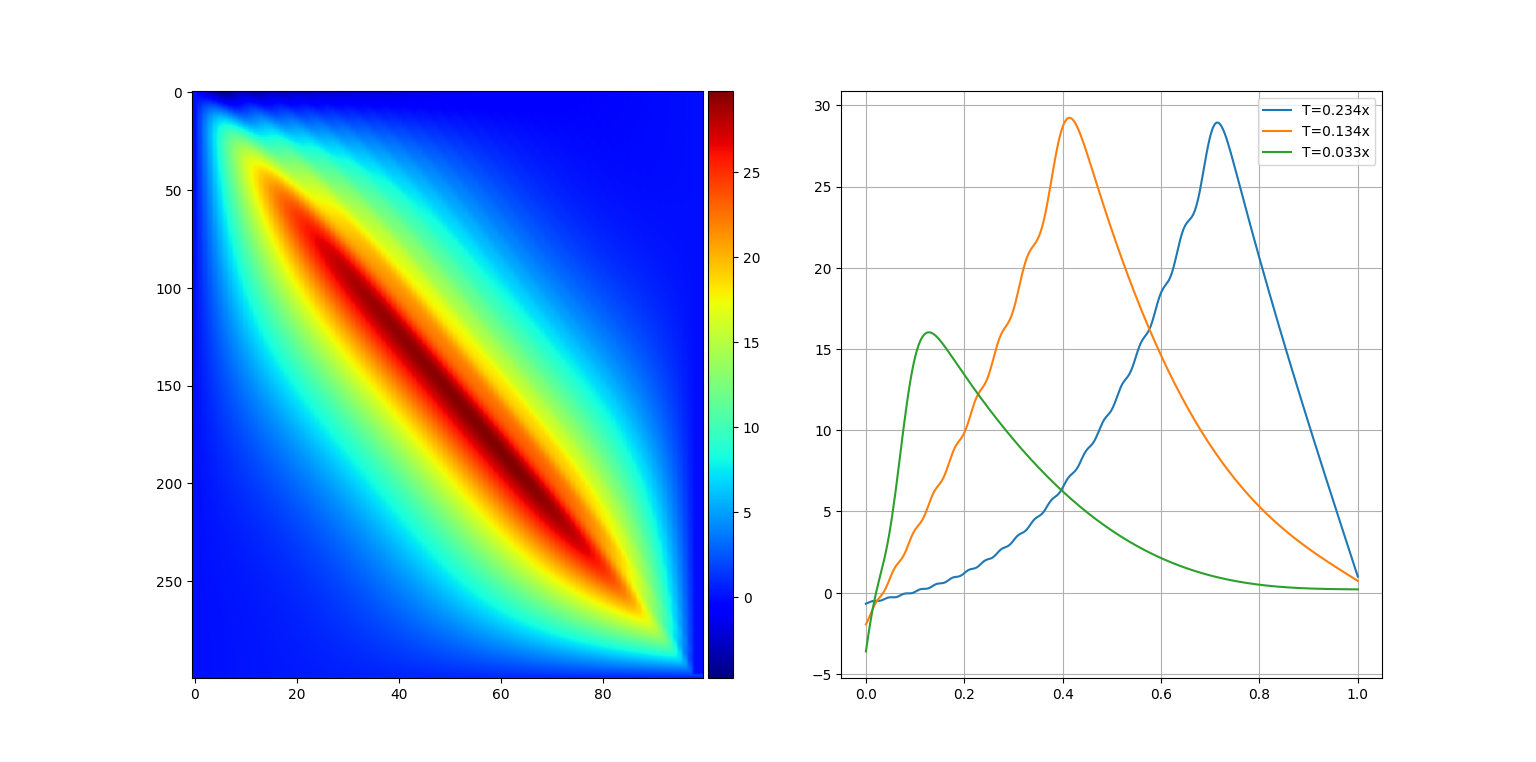
\includegraphics[width=\textwidth]{graph1.png}
    \end{figure}
    \newpage    
    \subsection{Problema 2}
    Grafique la función de onda, con los siguientes valores:
    \begin{quote}
        \centering
        \eq{a = 1}, \eq{b = 1}, \eq{v = 2}, \eq{f(x) = x^2 - x + sin(2x)} y \eq{g(x) = sin(x)}.
    \end{quote}
    \subsubsection{Programación}
    A continuación el \emph{main()} para el problema:

\begin{lstlisting}[frame=single]
def main():
    xf = 1#longitud final
    tf = 1#tiempo final
    v = 2#velocidad 
    #nx < nt
    #malla
    nx = 100#cols
    nt = 300#filas
    #condiciones frontera e iniciales
    f = lambda x: x**2 - x + m.sin(2*x)
    g = lambda x: m.sin(x)
    phi1 =lambda x: 0
    phi2 = lambda x: 0
    #ecuacion de onda
    ecuacionOnda(xf,tf,v,f,g,phi1,phi2,nx,nt)

if __name__ == "__main__":
    main()
\end{lstlisting}

    \subsubsection{Resultados}
    Se puede ver gracias a la gráfica izquierda que la onda tiene tendencia convexa, es decir, que
    tiende a hundirse hacia abajo(por debajo de 0), donde el punto más bajo estaria alrededor de -12.

    \begin{figure}[h]
        \centering
        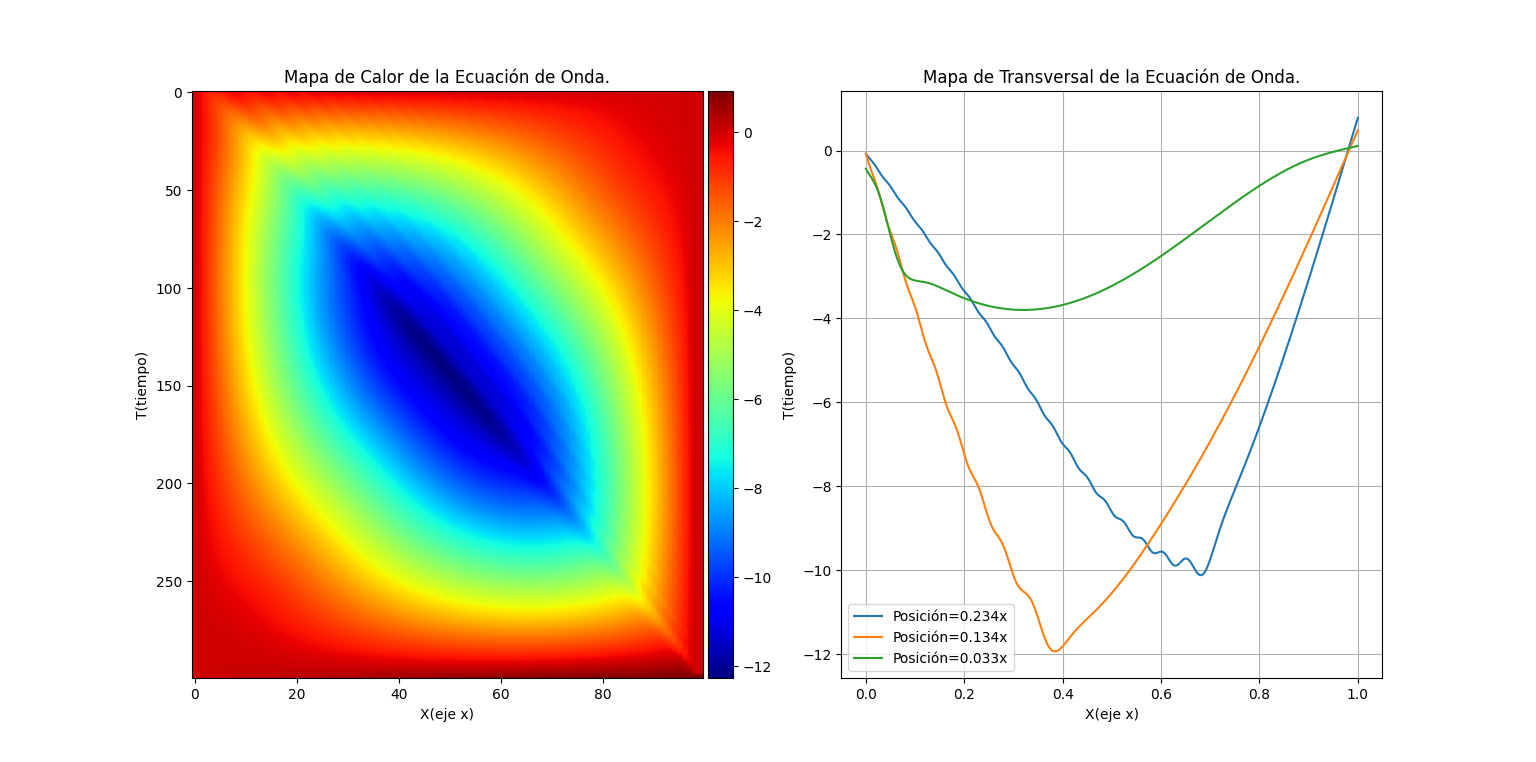
\includegraphics[width=\textwidth]{graph2.png}
    \end{figure}

    \subsection{Problema 3}
    Grafique la función de onda, con los siguientes valores:
    \begin{quote}
        \centering
        \eq{a = 1}, \eq{b = 1}, \eq{v = 1}, \eq{f(x) = sin(x)} y \eq{g(x) = 0}.
    \end{quote}
    \subsubsection{Programación}
    A continuación el \emph{main()} para el problema:

\begin{lstlisting}[frame=single]
def main():
    xf = 1#longitud final
    tf = 1#tiempo final
    v = 1#velocidad 
    #nx < nt
    #malla
    nx = 100#cols
    nt = 300#filas
    #condiciones frontera e iniciales
    f = lambda x: m.sin(x)
    g = lambda x: 0
    phi1 =lambda x: 0
    phi2 = lambda x: 0
    #ecuacion de onda
    ecuacionOnda(xf,tf,v,f,g,phi1,phi2,nx,nt)

if __name__ == "__main__":
    main()
\end{lstlisting}

    \subsubsection{Resultados}
    A continuación, en la gráfica izquierda, se modela como 
    gradualmente la onda es de forma convexa y que su punto más bajo 
    esta por debajo de -60.

    \begin{figure}[h]
        \centering
        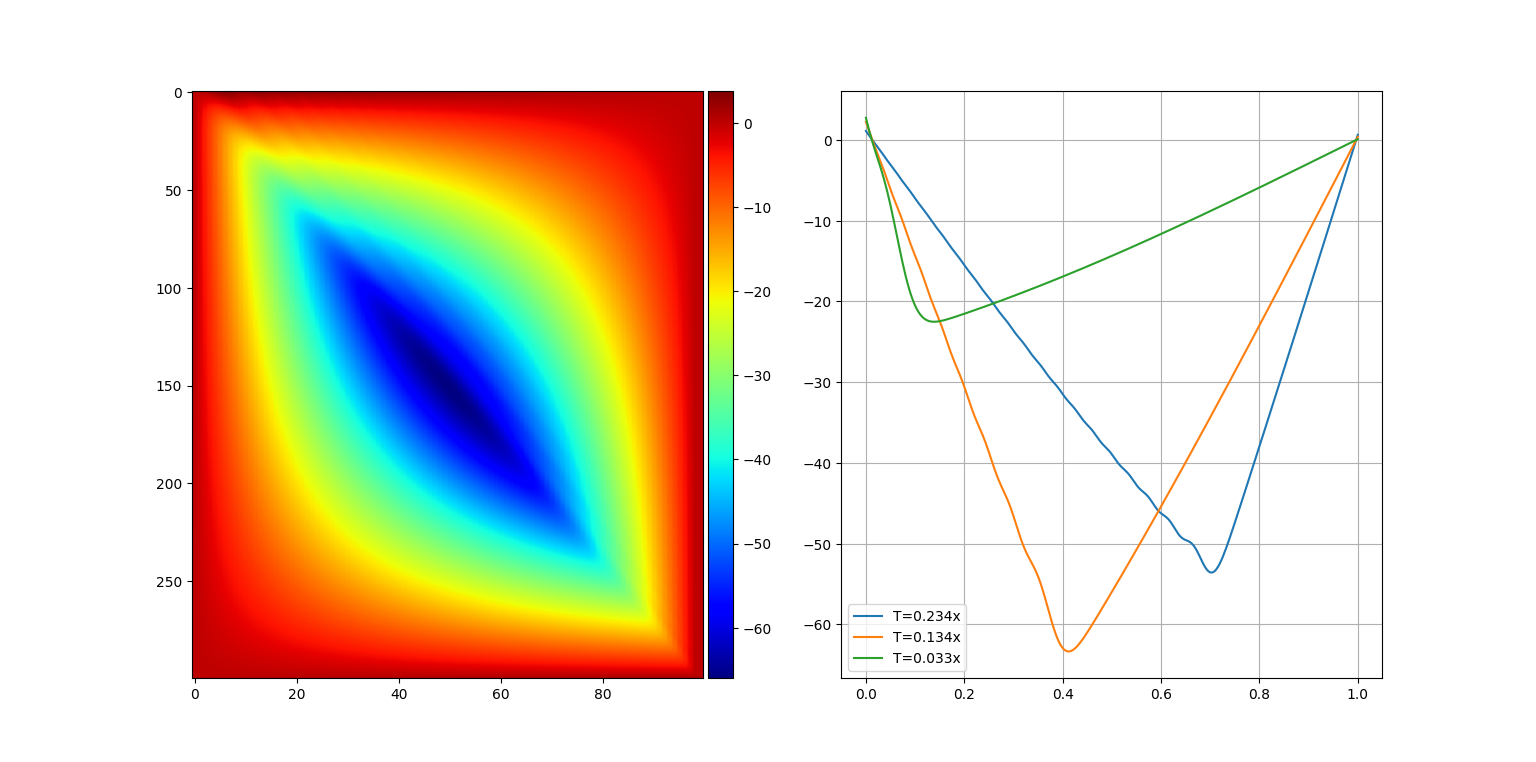
\includegraphics[width=\textwidth]{graph3.png}
    \end{figure}

    \subsection{Problema 4}
    Grafique la función de onda, con los siguientes valores:
    \begin{quote}
        \centering
        \eq{a = 1}, \eq{b = 1}, \eq{v = 1}, \eq{f(x) = 2x - 1} y \eq{g(x) = 0}.
    \end{quote}
    \subsubsection{Programación}
    A continuación el \emph{main()} para el problema:

\begin{lstlisting}[frame=single]
def main():
    xf = 1#longitud final
    tf = 1#tiempo final
    v = 1#velocidad 
    #nx < nt
    #malla
    nx = 100#cols
    nt = 300#filas
    #condiciones frontera e iniciales
    f = lambda x: 2*x-1
    g = lambda x: 0
    phi1 =lambda x: 0
    phi2 = lambda x: 0
    #ecuacion de onda
    ecuacionOnda(xf,tf,v,f,g,phi1,phi2,nx,nt)

if __name__ == "__main__":
    main()
\end{lstlisting}

    \subsubsection{Resultados}
    La ecuación de onda graficada en la siguiente imágen, muestra que en un tiempo de 1 segundo,
    se formaron 4 ondas, dos de la cuales son de forma convexa y las otras dos cóncavas.
    En la imagen izquierda se muestra los máximos y mínimos del desarrollo de la ecuacion de onda
    de las cuatro ondas.

    \begin{figure}[h]
        \centering
        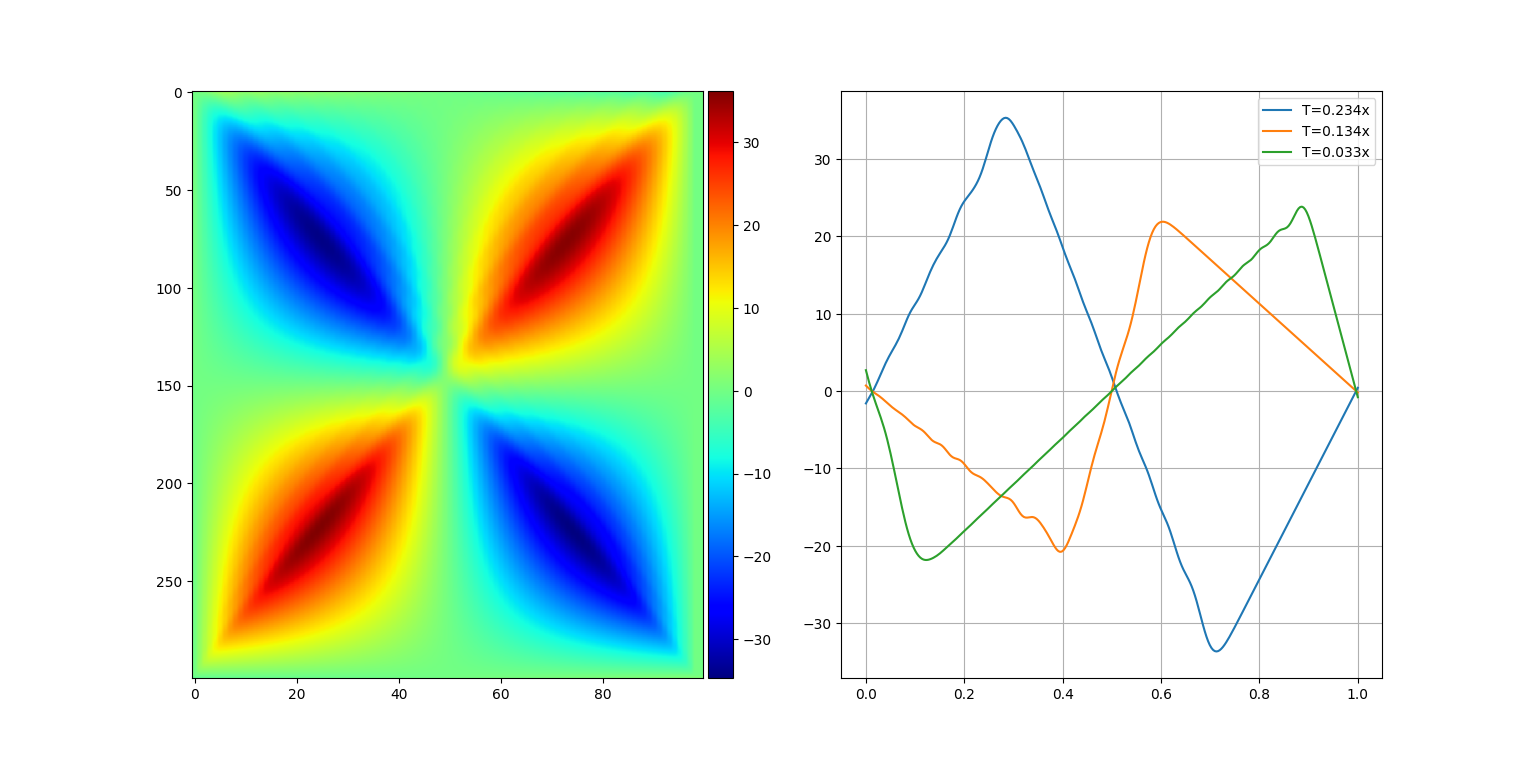
\includegraphics[width=\textwidth]{graph4.png}
    \end{figure}

    \subsection{Problema 5}
    Grafique la función de onda, con los siguientes valores:
    \begin{quote}
        \centering
        \eq{a = 1}, \eq{b = 1}, \eq{d = 1}, \eq{v = 1},\eq{f(x) = |4x - 1|} y \eq{g(x) = 0}.
    \end{quote}
    \subsubsection{Programación}
    A continuación el \emph{main()} para el problema:

\begin{lstlisting}[frame=single]
def main():
    xf = 1#longitud final
    tf = 1#tiempo final
    v = 1#velocidad 
    #nx < nt
    #malla
    nx = 100#cols
    nt = 300#filas
    #condiciones frontera e iniciales
    f = lambda x: abs(4*x-1)
    g = lambda x: 0
    phi1 =lambda x: 0
    phi2 = lambda x: 0
    #ecuacion de onda
    ecuacionOnda(xf,tf,v,f,g,phi1,phi2,nx,nt)

if __name__ == "__main__":
    main()
\end{lstlisting}

    \subsubsection{Resultados}
    Como se observa, la forma de la onda es convexa, y esta por dejajo de 0. 
    En la imagen izquierda se puede ver el progreso de la onda a traves del eje X, viendo 
    que aproximadamente el punto mínimo esta entre -150 y -175.
    \begin{figure}[h]
        \centering
        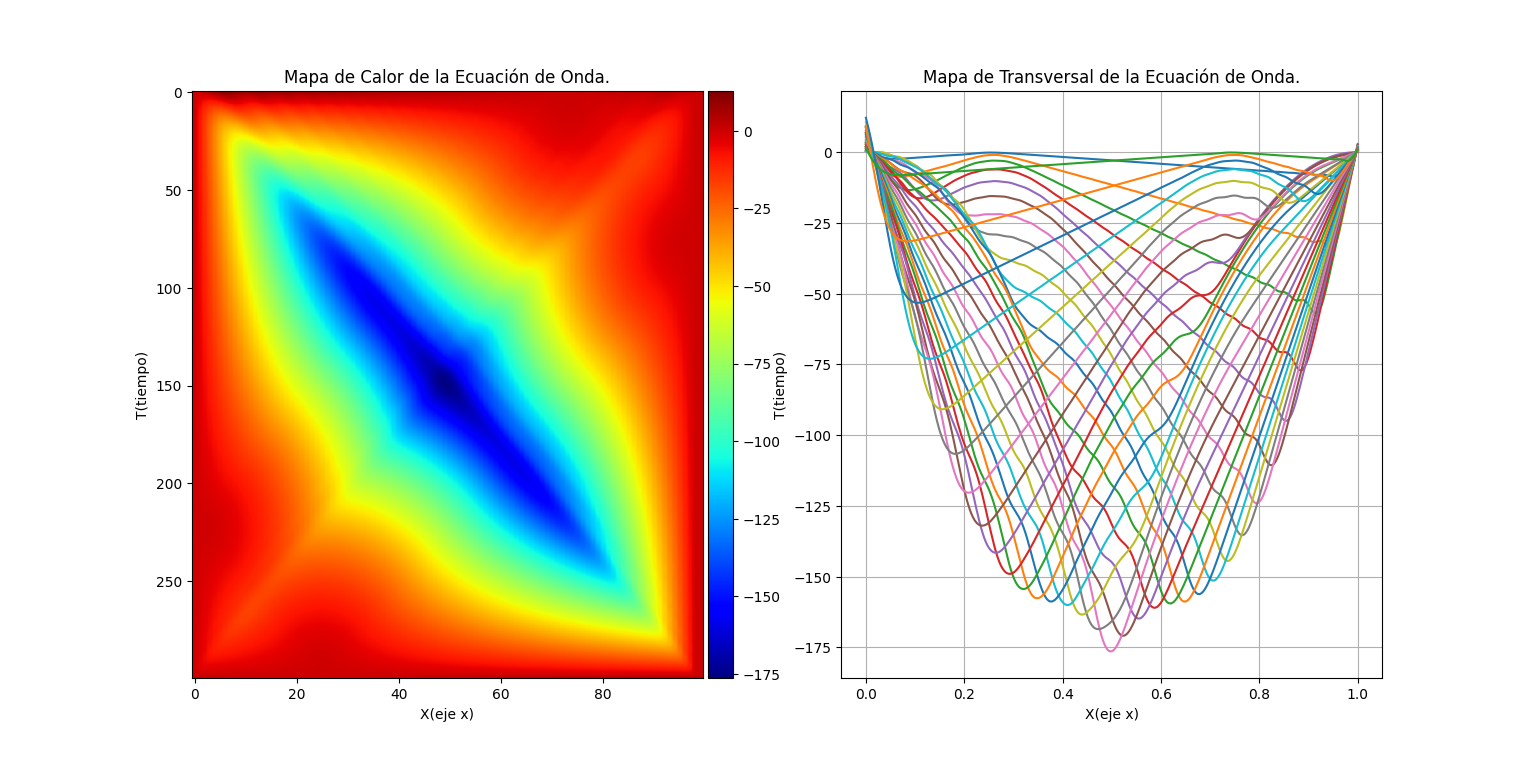
\includegraphics[width=\textwidth]{graph5.png}
    \end{figure}
    \section{Anexos}
    En el siguiente link están los archivos en Python:
    URL:\\ 
    \url{https://drive.google.com/drive/folders/1QtxLqNn8lSFFY1SxxB4cBQNLEMavW-SZ?usp=sharing}

\end{document}
